\documentclass[11pt]{article}

\usepackage{sectsty}
\usepackage{graphicx}
\usepackage{xcolor}
\usepackage{caption}
\usepackage[verbose]{placeins}

\usepackage[backend=biber, style=ieee, sorting=none, maxbibnames=99]{biblatex}

\DeclareFieldFormat
    [article,inbook,incollection,inproceedings,patent,thesis,
    unpublished,techreport,misc,book]
    {title}{\mkbibquote{#1}}  
\addbibresource{references.bib}

\graphicspath{{./images/}}

\topmargin=-0.45in
\evensidemargin=0in
\oddsidemargin=0in
\textwidth=6.5in
\textheight=9.0in
\headsep=0.25in

\title{\textbf{Documentation for the final project: \\ Collaboration between Human and AI in Typography}}
\author{Theodor Peifer \\ email: theodor.peifer@hm.edu \\ Hochschule München}
\date{\today}

\captionsetup[figure]{font=small}

\definecolor{blackColor}{HTML}{020202}
\definecolor{yellowColor}{HTML}{FFD100}

\begin{document}
\maketitle

\pagebreak

\section{Introduction}
Recent advances in the field of image generation using Artificial Intelligence allow individuals to create stunning images without any creative effort - including in the field of typography.
However, the use of generative AI in arts raises interesting questions about the role of the human in the creative process. On the one hand, the human is taking a passive role, simply providing the input data and allowing the AI to generate the final product. On the other hand, the human is actively participating in the design process: First by designing the AI itself, which requires a big amount of creative thought and effort and secondly by exploring and refining the results the model generated.
This process can be described as \emph{meta-creativity} \cite{metaCreativity}, where the individual only passively participates in the creative work, but instead actively invents creative ways to automate it.
In order to explore and reflect on this concept, an AI for generating new font styles will be developed, which will be displayed in a typographic manual. This article will contain a detailed documentation of this process.


\section{Methodology}
This project consists of three parts: Researching previous work about artificial font generation, developing the model and designing the typographic manual.
The research is done by searching and examining existing papers and their proposed methods. After determining the appropriate model for this problem, the next step is to gather the dataset. Then the model can be built and trained. Finally, the best results will be gathered and displayed in the manual, which is designed using \emph{Figma} \cite{figmaUIDesignTool}.


\section{Previous Work}
The state-of-the-art model for generating novel type faces has been developed by Hayashi et al. in their paper \emph{GlyphGAN: Style-Consistent Font Generation Based on Generative Adversarial Networks} \cite{glyphGan}. They propose the usage of a \emph{Generative Adversarial Network} \cite{gan} (GAN). A GAN consists of two neural networks: The generator and the discriminator. The generator learns to generate "fake" data from random noise and the discriminator network learns to classify between such fake data and real data. The goal of the generator is therefore to fool the discriminator by creating synthetic but realistic data. This model can be applied to generate fonts and will learn to produce 64x64 black and white images containing a single letter. In order to generate all letters in the alphabet in the same font style, the authors introduce style-consistency: Instead of feeding the generator just random noise, the input will consist of two concatenated vectors: A random style-vector and a vector which numerically represents a letter using one-hot encoding. To produce an alphabet with the same style over all letters, the style-vector has to be the same.
Similar work has been done by Erik Bernhardsson who developed the \emph{deep-fonts} \cite{deepFonts} font generator which used a simple dense neural network instead of a convolution based model.
A detailed comparison by Hayashi et al. proved that their method produces more consistent and legible glyphs. Therefore, this project employs a model heavily influenced by the \emph{GlyphGAN}.

\begin{figure}
    \centering
    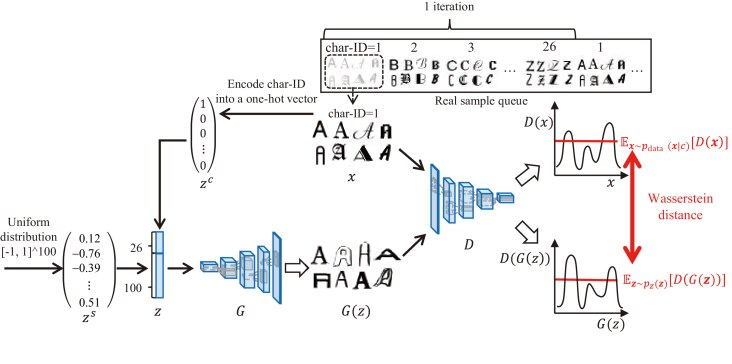
\includegraphics[width=0.75\columnwidth]{glyphgan.png}
    \caption{The GlypGAN architecture \cite{glyphGanImage}.}
    \label{fig:glyphgan}
\end{figure}

\section{Development of the Generative Model}
\subsection{The Dataset}
Since the dataset used to train the \emph{GlyphGAN} is not accessible, the model will be trained using the dataset collected by E. Bernhardsson for his \emph{deep-fonts} model which consists of 56443 different fonts scraped from the internet. Each font set consists of 62 characters. For simplicity and better results the model will only be trained on upper case letters and will therefore be able to create only such. When examining random samples of the dataset, it becomes obvious that there is a lot of noise present. Noise in this case meaning that some glyphs are handwritten or even unreadable which is expected to reduce the quality of the generated images. Yet, because of time and complexity issues the dataset has not been cleaned.

\subsection{The Model and Training}
The model was developed using the popular and powerful \emph{PyTorch} \cite{paszke2019pytorch} Deep Learning Framework for Python, which enables the implementation of complex architectures.
This stage of the project took around two weeks, since training a model took up to five hours and multiple training runs had to be done in order to find the optimal parameters. Although the final model wasn't able to reproduce as good results as shown in the GlyphGAN paper, the generated letters still had consistent font styles which could be used as inspiration for typographers.

\section{Design of the Typographic Manual}
\subsection{The Process}
The typographic manual consists of three sections: First comes an introduction that briefly explains the project, followed by a collection of alphabets, and finally a small explanation of how the AI works.
Designing it turned out to be a challenging task for the following reasons: First, the letters generated by the AI are in a low resolution pixel and not in a vector format, which is needed to be usable as a real font. Additionally, the letters are not pixel perfect, which means that there is often noise around the letter. And lastly, many glyphs are not legible (e.g. the model is barely able to produce the letter \emph{A} or \emph{S}) or look like other letters in the alphabet.
In order to still be able to display generated characters, the letter images have to be post-processed by hand and then recreated using vector shapes. To form whole words, images containing specific letters have to be concatenated. The letters displayed in the manual are chosen from the most interesting and most legible generated glyphs. But in order to show all of them, nine entire alphabets are shown in the manual.

\begin{figure}
    \centering
    
\includegraphics[width=0.5\columnwidth]{examples.png}
    \caption{Example of a noisy glyph, a collapsed glyph and a well generated glyph.}
    \label{fig:examples}
\end{figure}

\subsection{The Design}
The manual is designed using three colors: Black (\textcolor{blackColor}{\#020202}), yellow (\textcolor{yellowColor}{\#FFD100}) and white for the font color. Each black page, which contains the primary content such as text and alphabets, is followed by a yellow page displaying a generated letter or word. The font \emph{Sulphur Point} is used for the text and titles. Since the AI can only generate upper case letters, the entire text is also chosen to be in upper case in order to maintain consistency.
Constellations of small, yellow squares are used as a recurring theme. By arranging them in a rectangular shape and giving them depth through a shadow, they represent multidimensional matrices and vectors which are being used for machine learning calculations.

\begin{figure}[hbt!]
    \centering
    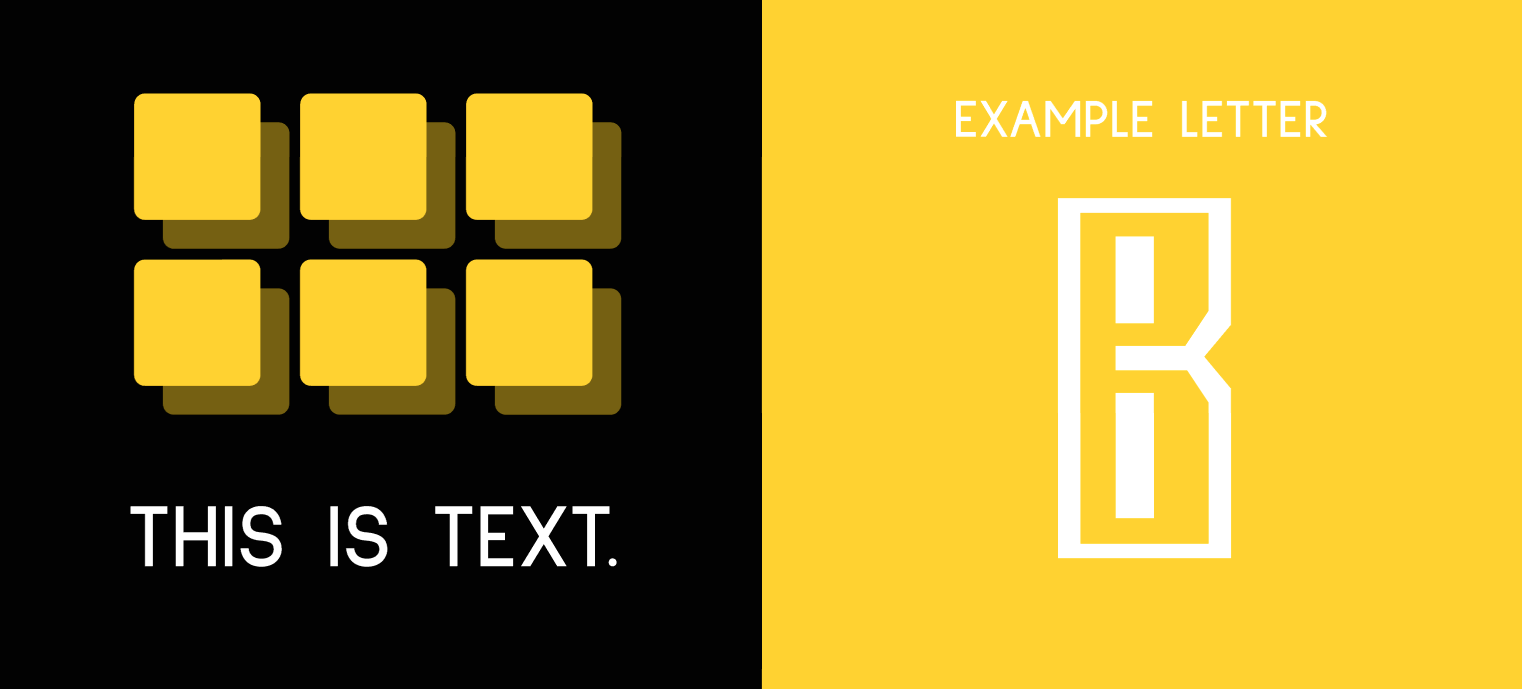
\includegraphics[width=0.75\columnwidth]{design.png}
    \caption{Example of the design elements.}
    \label{fig:design}
\end{figure}
\FloatBarrier

\section{Conclusion}
This project has shown that generative AI can significantly improve the quantity and time efficiency of typographic work. In seconds, the model can develop different types of typefaces, but lacks the precision of human work. Even though humans can still be creative through the development and use of AI, it takes away the possibility of creativity from those who work in the field where the AI is being used - in this case, typography. It's crucial to find a balance between utilizing the benefits of generative AI while also valuing and preserving the creativity of human artists.
The code and the typographic manual can be found in the GitHub repository \cite{fontGenerationGan} of this project.

\begin{figure}[hbt!]
    \centering
    
\includegraphics[width=0.35\columnwidth]{font_examples.png}
    \caption{Example of words using generated fonts.}
    \label{fig:font_examples}
\end{figure}
\FloatBarrier

\printbibliography

\end{document}